\documentclass[12pt]{article}
\usepackage{amsmath}
\usepackage{graphicx}
\usepackage{hyperref}
\usepackage{listings}
\usepackage{color}
\usepackage{pythonhighlight}

\title{Operating System Course Report - First Half of the Semester}
\author{A class}
\date{\today}

\begin{document}

\maketitle
\newpage

\tableofcontents
\newpage

\section{Introduction}
This report summarizes the topics covered during the first half of the Operating System course. It includes theoretical concepts, practical implementations, and assignments. The course focuses on the fundamentals of operating systems, including system architecture, process management, CPU scheduling, and deadlock handling.

\section{Course Overview}
\subsection{Objectives}
The main objectives of this course are:
\begin{itemize}
    \item To understand the basic components and architecture of a computer system.
    \item To learn process management, scheduling, and inter-process communication.
    \item To explore file systems, input/output management, and virtualization.
    \item To study the prevention and handling of deadlocks in operating systems.
\end{itemize}

\subsection{Course Structure}
The course is divided into two halves. This report focuses on the first half, which covers:
\begin{itemize}
    \item Basic Concepts and Components of Computer Systems
    \item System Performance and Metrics
    \item System Architecture of Computer Systems
    \item Process Description and Control
    \item Scheduling Algorithms
    \item Process Creation and Termination
    \item Introduction to Threads
    \item File Systems
    \item Input and Output Management
    \item Deadlock Introduction and Prevention
    \item User Interface Management
    \item Virtualization in Operating Systems
\end{itemize}

\section{Topics Covered}

\subsection{Basic Concepts and Components of Computer Systems}
This section explains the fundamental components that make up a computer system, including the CPU, memory, storage, and input/output devices.

\subsection{System Performance and Metrics}
\subsubsection{Metrik Sistem Spesifik}
\begin{enumerate}
    \item \textit{Cycle Per Instructions} (CPI) 
    \par \textit{Cycle Per Instructions} adalah salah satu metrik utama yang digunakan untuk mengevaluasi performa \textit{Central Processing Unit} (CPU). CPI mengukur rata-rata jumlah siklus \textit{clock} yang dibutuhkan oleh CPU untuk mengeksekusi satu instruksi.
    \par Formula umum CPI: 
    \par CPI = \textit{Total Cycle/Instructions}
    \par Rendahnya CPI berarti CPU dapat mengeksekusi instruksi lebih efisien, menunjukkan performa yang lebih baik sedangkan tingginya CPI menunjukkan bahwa CPU memerlukan lebih banyak siklus \textit{clock} untuk mengeksekusi instruksi, yang bisa berarti instruksi tersebut lebih kompleks atau ada masalah dalam \textit{pipeline} CPU.
    \par Contoh Penggunaan CPI
    \par Misalkan kamu memiliki dua CPU: 
    \par CPU A memiliki CPI 1.2 
    \par CPU B memiliki CPI 1.8 
    \par Jika keduanya berjalan pada frekuensi yang sama, katakanlah 3 GHz, CPU A akan lebih efisien karena membutuhkan lebih sedikit siklus per instruksi. Ini berarti CPU A dapat menyelesaikan lebih banyak instruksi dalam waktu yang sama dibandingkan CPU B.

    \item \textit{Floating Point Operations Per Second} (FLOPS)
    \par \textit{Floating Point Operations Per Second} adalah metrik yang digunakan untuk mengukur
    kemampuan komputasi \textit{floating-point} dari sebuah
    komputer, yang sangat penting dalam aplikasi yang
    memerlukan kalkulasi numerik berat, seperti simulasi
    ilmiah, pemodelan 3D, atau \textit{machine learning}.
    \par Contoh Penggunaan FLOPS:
    \par Bayangkan kamu bekerja di bidang simulasi ilmiah yang memerlukan perhitungan numerik yang intensif. Sistem A memiliki kapasitas 2 TFLOPS, sementara Sistem B memiliki 5 TFLOPS. Sistem B akan mampu menyelesaikan simulasi tersebut lebih cepat, karena dapat melakukan lebih banyak operasi \textit{floating-point} per detik.

    \item \textit{Input/Output Operations Per Second} (IOPS)
    \par \textit{Input/Output Operations Per Second} mengukur performa dari perangkat penyimpanan (seperti SSD, HDD) dalam hal jumlah operasi \textit{input/output} yang dapat diproses dalam satu detik. IOPS sering digunakan untuk mengevaluasi performa \textit{disk} dan sistem penyimpanan.
    \par Contoh Penggunaan IOPS:
    \par Misalkan kamu mengelola \textit{server database}. SSD A memiliki 100,000 IOPS, sementara SSD B memiliki 50,000 IOPS. SSD A akan mampu menangani lebih banyak operasi baca/tulis per detik, sehingga lebih cocok untuk lingkungan \textit{database} yang memerlukan akses data cepat dan simultan.
    
\end{enumerate}


\subsection{System Architecture of Computer Systems}
Describes the architecture of modern computer systems, focusing on the interaction between hardware and the operating system.

\subsection{Process Description and Control}
Processes are a central concept in operating systems. This section covers:
\begin{itemize}
    \item Process states and state transitions
    \item Process control block (PCB)
    \item Context switching
\end{itemize}

\subsection{Scheduling Algorithms}
This section covers:
\begin{itemize}
    \item First-Come, First-Served (FCFS)
    \item Shortest Job Next (SJN)
    \item Round Robin (RR)
\end{itemize}
It explains how these algorithms are used to allocate CPU time to processes.

\subsection{Process Creation and Termination}
Details how processes are created and terminated by the operating system, including:
\begin{itemize}
    \item Process spawning
    \item Process termination conditions
\end{itemize}

\subsection{Introduction to Threads}
This section introduces the concept of threads and their relation to processes, covering:
\begin{itemize}
    \item Single-threaded vs. multi-threaded processes
    \item Benefits of multithreading
\end{itemize}

\begin{figure}[h]
    \centering
    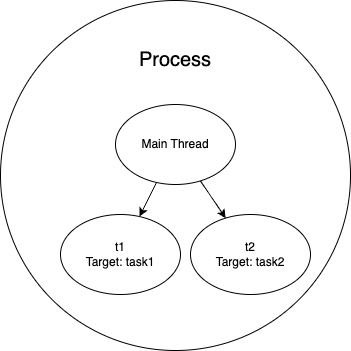
\includegraphics[width=0.5\textwidth]{/Users/khawaritzmi/Unhas/os_report_mid2024/a_class/asset/example.png}  % Sesuaikan nama file dan ukurannya
    \caption{Ini adalah gambar contoh dari multithreading.}
    \label{fig:contoh_gambar}
\end{figure}

Seperti yang terlihat pada Gambar \ref{fig:contoh_gambar}, inilah cara menambahkan gambar dengan keterangan.

\subsection{File Systems}
File systems provide a way for the operating system to store, retrieve, and manage data. This section explains:
\begin{itemize}
    \item File system structure
    \item File access methods
    \item Directory management
\end{itemize}

\subsection{Input and Output Management}
Input and output management is key for handling the interaction between the system and external devices. This section includes:
\begin{itemize}
    \item Device drivers
    \item I/O scheduling
\end{itemize}

\subsection{Deadlock Introduction and Prevention}
Explores the concept of deadlocks and methods for preventing them:
\begin{itemize}
    \item Deadlock conditions
    \item Deadlock prevention techniques
\end{itemize}

\subsection{User Interface Management}
This section discusses the role of the operating system in managing the user interface. Topics covered include:
\begin{itemize}
    \item Graphical User Interface (GUI)
    \item Command-Line Interface (CLI)
    \item Interaction between the user and the operating system
\end{itemize}

\subsection{Virtualization in Operating Systems}
Virtualization allows multiple operating systems to run concurrently on a single physical machine. This section explores:
\begin{itemize}
    \item Concept of virtualization
    \item Hypervisors and their types
    \item Benefits of virtualization in modern computing
\end{itemize}

\section{Assignments and Practical Work}
\subsection{Assignment 1: Process Scheduling}
Students were tasked with implementing various process scheduling algorithms (e.g., FCFS, SJN, and RR) and comparing their performance under different conditions.
\subsubsection{Group 1}
\begin{python}
    class Process:
    def __init__(self, pid, arrival_time, burst_time):
        self.pid = pid
        self.arrival_time = arrival_time
        self.burst_time = burst_time
        self.completion_time = 0
        self.turnaround_time = 0
        self.waiting_time = 0
\end{python}

\begin{table}[htbp] % Optional: For floating position
    \centering
    \begin{tabular}{|c|c|c|} % Defines number of columns and alignment (c = center, l = left, r = right). '|' creates vertical lines.
    \hline
    Header 1 & Header 2 & Header 3 \\ % Column headers
    \hline
    Row 1, Column 1 & Row 1, Column 2 & Row 1, Column 3 \\ % First row of data
    \hline
    Row 2, Column 1 & Row 2, Column 2 & Row 2, Column 3 \\ % Second row of data
    \hline
    \end{tabular}
    \caption{Your table caption} % Optional: For adding a caption
    \label{tab:your_label} % Optional: For cross-referencing the table
\end{table}
\subsection{Assignment 2: Deadlock Handling}
\subsubsection{Grup 2}
    \textbf{Soal:}
    \par Buatlah sebuah program Python sederhana yang mensimulasikan beberapa skenario deadlock dan mengeksplorasi berbagai metode pencegahan deadlock. Program ini harus mendukung beberapa fitur berikut:
    \begin{itemize}
    \item Simulasi skenario deadlock dengan penggunaan dua atau lebih sumber daya oleh beberapa proses.
    \item Implementasi metode pencegahan deadlock seperti pengurutan sumber daya, batasan jumlah maksimum sumber daya yang dapat dialokasikan, atau penggunaan algoritma Banker's.
    \item Visualisasi atau laporan mengenai status deadlock dan bagaimana pencegahannya dapat diterapkan.
    \item Tampilkan hasil dari skenario deadlock yang disimulasikan dan solusi pencegahannya.
    \end{itemize}

    \textbf{Jawaban:} \par Untuk menjawab soal ini, kita akan membuat program Python sederhana yang mensimulasikan skenario deadlock serta menerapkan metode pencegahannya. Berikut adalah implementasi dari program tersebut:
    \begin{python}
    import threading
    import time
    
    # Simulasi sumber daya
    class SumberDaya:
        def __init__(self, nama):
            self.nama = nama
            self.lock = threading.Lock()
    
    def gunakan(self, pengguna):
        with self.lock:
            print(f"{pengguna} menggunakan {self.nama}.")
            time.sleep(1)  # Simulasi waktu penggunaan sumber daya

    # Fungsi untuk simulasi deadlock
    def deadlock_scenario(sumber1, sumber2, pengguna):
        print(f"{pengguna} mencoba mengakses {sumber1.nama}.")
        sumber1.gunakan(pengguna)
    
        print(f"{pengguna} mencoba mengakses {sumber2.nama}.")
        sumber2.gunakan(pengguna)
    
    # Pencegahan deadlock: mengatur urutan pengaksesan sumber daya
    def no_deadlock_scenario(sumber1, sumber2, pengguna):
        sumber_list = sorted([sumber1, sumber2], key=lambda s: s.nama)
        
        print(f"{pengguna} mencoba mengakses {sumber_list[0].nama}.")
        sumber_list[0].gunakan(pengguna)
    
        print(f"{pengguna} mencoba mengakses {sumber_list[1].nama}.")
        sumber_list[1].gunakan(pengguna)
    
    def main():
        # Membuat sumber daya
        sumber_a = SumberDaya('SumberA')
        sumber_b = SumberDaya('SumberB')

    # Simulasi deadlock
    thread1 = threading.Thread(target=deadlock_scenario, args=(sumber_a, sumber_b, "Proses1"))
    thread2 = threading.Thread(target=deadlock_scenario, args=(sumber_b, sumber_a, "Proses2"))

    print("\nSimulasi Deadlock:")
    thread1.start()
    thread2.start()
    
    thread1.join()
    thread2.join()

    # Simulasi tanpa deadlock dengan pengurutan akses sumber daya
    print("\nSimulasi Pencegahan Deadlock:")
    thread3 = threading.Thread(target=no_deadlock_scenario, args=(sumber_a, sumber_b, "Proses1"))
    thread4 = threading.Thread(target=no_deadlock_scenario, args=(sumber_b, sumber_a, "Proses2"))

    thread3.start()
    thread4.start()
    
    thread3.join()
    thread4.join()

    if __name__ == "__main__":
        main()

    \end{python}
\subsection{Assignment 3: Multithreading and Amdahl's Law}
\subsubsection{Grup 2}
    \textbf{Soal:}
    \par Buatlah sebuah program Python yang mensimulasikan skenario multithreading untuk menyelesaikan masalah komputasi intensif. Setelah itu, terapkan Hukum Amdahl untuk menghitung kecepatan teoretis program tersebut ketika jumlah thread ditingkatkan. Program harus memenuhi beberapa kriteria berikut:
    \begin{itemize}
    \item Selesaikan masalah komputasi intensif (misalnya, penjumlahan bilangan dalam rentang besar) menggunakan beberapa thread.
    \item Hitung waktu eksekusi untuk setiap jumlah thread yang digunakan.
    \item Terapkan Hukum Amdahl untuk menghitung kecepatan teoretis ketika menambah jumlah thread.
    \item Bandingkan hasil teoritis dan hasil nyata dari waktu eksekusi program.
    \end{itemize}
    
    \textbf{Jawaban:}
    \par Berikut adalah implementasi program yang menggunakan multithreading untuk menyelesaikan masalah komputasi intensif, diikuti dengan perhitungan kecepatan teoretis menggunakan Hukum Amdahl:
    \begin{python}
    import threading
    import time
    import os

    # Fungsi komputasi intensif: penjumlahan bilangan dari 1 hingga N
    def komputasi_intensif(n, hasil, index):
        total = 0
        for i in range(1, n+1):
            total += i
        hasil[index] = total
        print(f"Thread-{index+1} selesai, hasil: {total}")

    # Fungsi untuk menghitung waktu eksekusi menggunakan multithreading
    def hitung_waktu_multithreading(n, jumlah_thread):
        hasil = [0] * jumlah_thread
        threads = []
        bagian = n // jumlah_thread

        start_time = time.time()

        for i in range(jumlah_thread):
            batas_atas = (i+1) * bagian if i != jumlah_thread - 1 else n
            t = threading.Thread(target=komputasi_intensif, args=(batas_atas, hasil, i))
            threads.append(t)
            t.start()

        for t in threads:
            t.join()

        end_time = time.time()

        total_hasil = sum(hasil)
        waktu_eksekusi = end_time - start_time
        print(f"Total hasil: {total_hasil}, Waktu eksekusi dengan {jumlah_thread} thread: {waktu_eksekusi:.4f} detik")
        return waktu_eksekusi

    # Hukum Amdahl: menghitung kecepatan teoretis
    def hitung_kecepatan_teoretis(serial_fraction, jumlah_thread):
        return 1 / (serial_fraction + (1 - serial_fraction) / jumlah_thread)

    def main():
        n = 10**7  # Besar masalah (penjumlahan hingga N)
        jumlah_threads = [1, 2, 4, 8]  # Daftar jumlah thread yang akan diuji
        serial_fraction = 0.1  # Asumsi fraksi yang tidak bisa diparalelkan (10%)

        waktu_eksekusi_awal = None

        # Bandingkan waktu eksekusi dengan jumlah thread yang berbeda
        for thread_count in jumlah_threads:
            waktu_eksekusi = hitung_waktu_multithreading(n, thread_count)

            if thread_count == 1:
                waktu_eksekusi_awal = waktu_eksekusi  # Simpan waktu eksekusi serial (1 thread)

            # Hitung kecepatan teoretis menggunakan Hukum Amdahl
            kecepatan_teoretis = hitung_kecepatan_teoretis(serial_fraction, thread_count)
            print(f"Kecepatan teoretis dengan {thread_count} thread: {kecepatan_teoretis:.4f}x")

            # Hitung kecepatan nyata berdasarkan hasil eksekusi
            kecepatan_nyata = waktu_eksekusi_awal / waktu_eksekusi
            print(f"Kecepatan nyata dengan {thread_count} thread: {kecepatan_nyata:.4f}x\n")

    if __name__ == "__main__":
        main()

        \end{python}

\subsection{Assignment 4: Simple Command-Line Interface (CLI) for User Interface Management}
Students were tasked with creating a simple **CLI** for user interface management. The CLI should support basic commands such as file manipulation (creating, listing, and deleting files), process management, and system status reporting.

\subsection{Assignment 5: File System Access}
In this assignment, students implemented file system access routines, including:
\begin{itemize}
    \item File creation and deletion
    \item Reading from and writing to files
    \item Navigating directories and managing file permissions
\end{itemize}

\section{Conclusion}
The first half of the course introduced core operating system concepts, including process management, scheduling, multithreading, and file system access. These topics provided a foundation for more advanced topics to be covered in the second half of the course.

\end{document}